\section{Modelo DEVS Acoplado}

El sistema completo se modela mediante un DEVS acoplado:
\[
N = \left< X_N,\, Y_N,\, D,\, \{M_d\},\, EIC,\, EOC,\, IC,\, Select \right>
\]

donde:
\[
D = \{ M_{gen}, M_{ctrl}, M_{bomba}, M_{sensor}, M_{alarmas}, M_{logger}, M_{bolsa}, M_{enf} \}
\]

\subsection{Definición formal}

\paragraph{Puertos externos.}
\[
X_N = \varnothing
\]
\[
Y_N = \{ \mathrm{alarmaBaja}, \mathrm{alarmaMedia}, \mathrm{alarmaCritica} \} \times \{0\}
\]

\paragraph{Acoplamientos de entrada y salida externa.}
\[
EIC = \varnothing
\]
\[
EOC = \{ [(M_{alarmas},0),(N,0)] \}
\]

\paragraph{Acoplamientos internos.}
\[
IC = \{
[(M_{gen},0),(M_{ctrl},0)],\;
[(M_{gen},0),(M_{bolsa},0)],\;
[(M_{gen},0),(M_{enf},0)],\; \dots
\}
\]
El lazo cerrado de control se implementa como: $Controlador \rightarrow Bomba \rightarrow Sensor \rightarrow Controlador$.

\paragraph{Función de desempate.}
Para resolver eventos simultáneos se define una prioridad fija entre modelos:
\[
M_{gen} > M_{ctrl} > M_{bomba} > M_{sensor} > M_{bolsa} > M_{enf} > M_{alarmas} > M_{logger}
\]
Por lo tanto:
\[
Select(H) = \text{el primer elemento de } H \text{ según el orden anterior}
\]

\subsection{Diagrama de acoplamiento}

\begin{figure}[htbp]
    \centering
    % Aquí se ajustó el width a 0.85\textwidth para que no desborde los márgenes visuales
    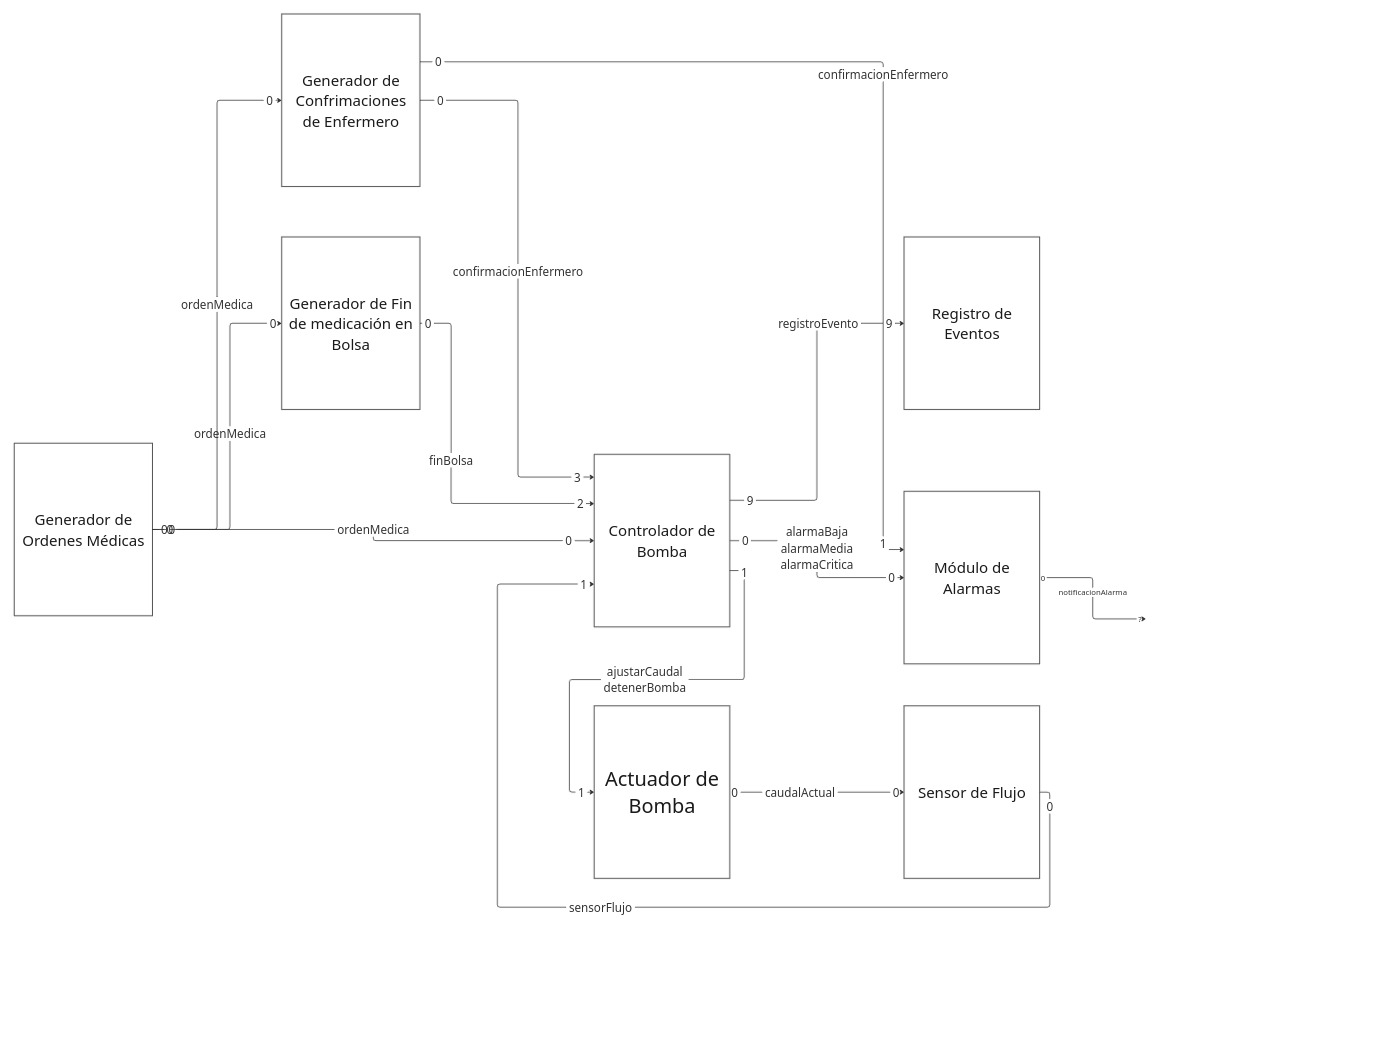
\includegraphics[width=0.85\textwidth]{devs_version_5.jpg} 
    \caption{Diagrama de acoplamiento del sistema de bomba de infusión.}
    \label{fig:diagrama_acoplado}
\end{figure}